\documentclass[12pt,a4paper]{book}
\usepackage[utf8]{inputenc}
\usepackage[brazil]{babel}
\usepackage[T1]{fontenc}
\usepackage{amsmath}
\usepackage{amsfonts}
\usepackage{amssymb}
\usepackage{makeidx}
\usepackage{graphicx}
\usepackage[all]{xy}
\usepackage{float}
\usepackage[left=2cm,right=2cm,top=2cm,bottom=2cm]{geometry}
\DeclareMathOperator{\sen}{sen}
\DeclareMathOperator{\cossec}{cossec}
\DeclareMathOperator{\tg}{tg}
\title{Pré-Cálculo}


\begin{document}

%titulo
\maketitle

%sumario
\tableofcontents

\chapter{Conjuntos}

\section{Noção de Conjunto}


Um conjunto é uma coleção qualquer de objetos formado por elementos. Um objeto \textbf{a} qualquer pode ser elemento de determinado conjunto $A$ ou não.


\begin{center}
	Quando \textbf{a} pertençe a $A$ escrevemos:
\end{center}
 	$$a \in A$$
 	
\begin{center}
	Quando \textbf{a} não pertençe a $A$ escrevemos:
\end{center}
	$$a \not\in A$$
	
	
\section{Conjuntos Númericos}

\subsection{Conjunto  dos Números Naturais $\mathbb{N}$}

O conjunto dos números naturais, simbolizado por $\mathbb{N}$ é o seguinte conjunto:

$$\mathbb{N} = \{0 \, ; \, 1\, ; \,2\, ; \,3\, ; \,4\,; \, ...\}$$

\textbf{Observações:}
\begin{itemize}
\item Quando $0 \not\in \mathbb{N}$ escrevemos $\mathbb{N}^*$.
$$\mathbb{N}^* = \{ 1\, ; \,2\, ; \,3\, ; \,4\, ; \, ...\}$$

\end{itemize}

\subsection{Conjunto  dos Números Inteiros $\mathbb{Z}$}

O conjunto dos números inteiros, simbolizado por $\mathbb{Z}$ é o seguinte conjunto:

$$\mathbb{Z} = \{...\,;\,-4\,;\,-3\,;\,-2\,;\,-1\,;\,0 \, ; \, 1\, ; \,2\, ; \,3\, ; \,4\, ; \, ...\}$$


\subsection{Conjunto  dos Números Racionais $\mathbb{Q}$}

O conjunto dos números racionais, simbolizado por $\mathbb{Q}$ é o conjunto das frações $\dfrac{a}{b}$ tal que $a \in \mathbb{Z}$ e $b \in \mathbb{Z}^*$.

$$\mathbb{Q} = \{...\,;\,-2\,;\,-1\,;\, -\frac{1}{2} \,;\,0 \, ; \, 1\, ;\,\frac{3}{2} \,; \,2\,; \, ...\}$$
\subsection{Conjunto  dos Números Irracionais $\mathbb{I}$}

O conjunto dos números irracionais, simbolizado por $\mathbb{I}$ é o conjunto dos números cuja representação com infinitas casas decimais não é periódica. Exemplo: $\sqrt{2};\,\sqrt{3};\,\pi$


\subsection{Conjunto  dos Números Reais $\mathbb{R}$}

O conjunto dos números reais, simbolizado por $\mathbb{R}$ é o conjunto formado por todos os números com representação decimal, decimais exatas e periódicas e as decimais não exatas e não periódicas.
\begin{figure}[H]
	\centering
	
	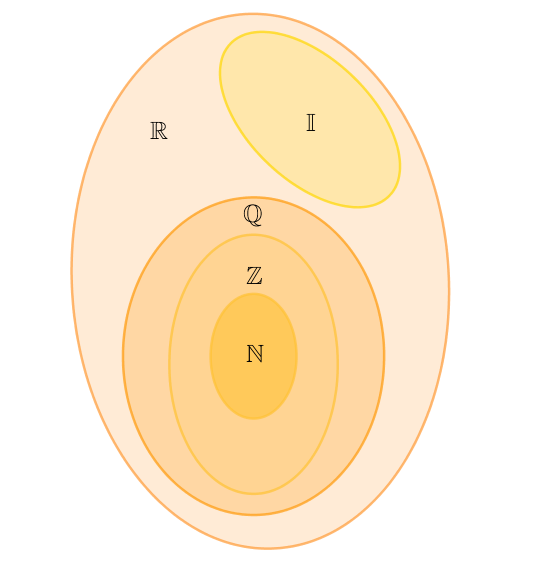
\includegraphics[scale=3.5]{imagens/conjunto-reais.png}

\end{figure}


\section{Intervalos Reais}

Dados dois números reais, $a$ e $b$, com $a < b$, temos:
\begin{itemize}
\begin{center}
	 Intervalo aberto
\end{center}

$$]a,b[ = \{x \in \mathbb{R}|\, a < x < b \}$$
\begin{figure}[H]
	\centering
	
	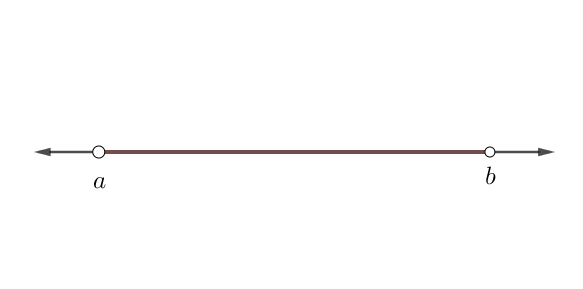
\includegraphics[scale=3.5]{imagens/intervalo-aberto.png}

\end{figure}

\begin{center}
	Intervalo fechado
\end{center}

$$[a,b] = \{x \in \mathbb{R}|\, a \leq x \leq b \}$$
\begin{figure}[H]
	\centering
	
	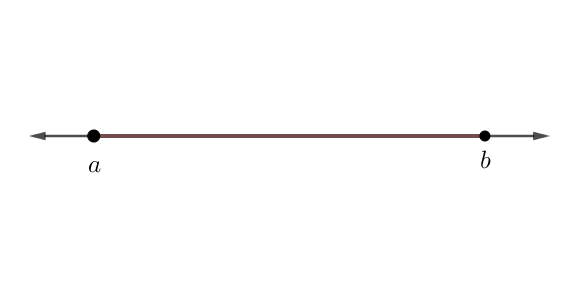
\includegraphics[scale=3.5]{imagens/intervalo-fechado.png}

\end{figure}
\begin{center}
	Intervalo fechado à esquerda e aberto à direita
\end{center}

$$[a,b[ = \{x \in \mathbb{R}|\, a \leq x < b \}$$
\begin{figure}[H]
	\centering
	
	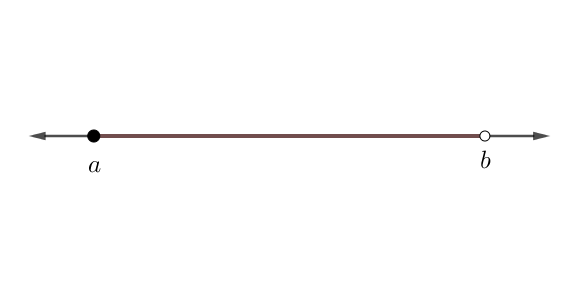
\includegraphics[scale=3.5]{imagens/intervalo-fechado-esquerda.png}

\end{figure}

\begin{center}
	Intervalo fechado à direita e aberto à esquerda
\end{center}

$$]a,b] = \{x \in \mathbb{R}|\, a < x \leq b \}$$
\begin{figure}[H]
	\centering
	
	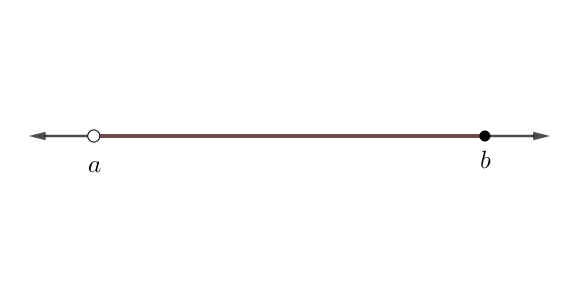
\includegraphics[scale=3.5]{imagens/intervalo-fechado-direita.png}

\end{figure}

\begin{center}
	Semirreta esquerda, fechada, de origem $b$
\end{center}

$$]-\infty,b] = \{x \in \mathbb{R}|\,  x \leq b \}$$
\begin{figure}[H]
	\centering
	
	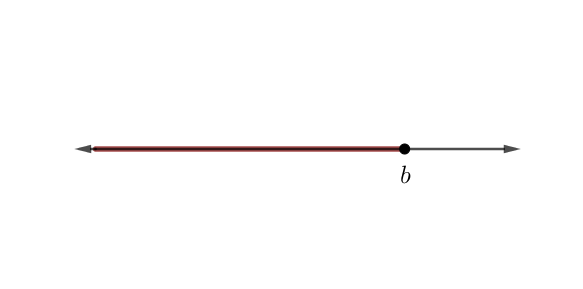
\includegraphics[scale=3.5]{imagens/semi-b-esquerda-fechada.png}

\end{figure}

\begin{center}
	Semirreta esquerda, aberta, de origem $b$
\end{center}

$$]-\infty,b[ = \{x \in \mathbb{R}|\,  x < b \}$$
\begin{figure}[H]
	\centering
	
	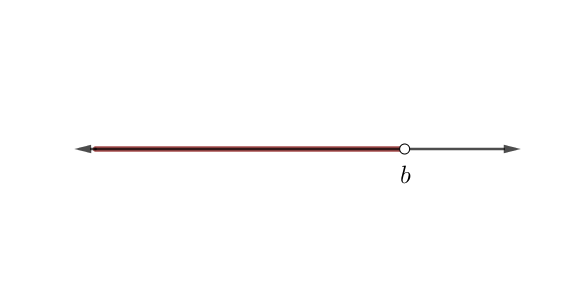
\includegraphics[scale=3.5]{imagens/semi-b-esquerda-aberta.png}

\end{figure}
\begin{center}
	Semirreta direita, fechada, de origem $a$
\end{center}

$$[a,+\infty[ = \{x \in \mathbb{R}|\,  x \geq a \}$$
\begin{figure}[H]
	\centering
	
	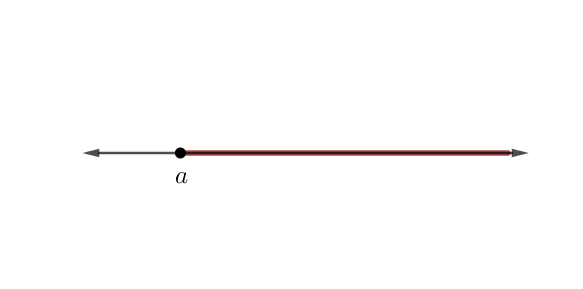
\includegraphics[scale=3.5]{imagens/semi-a-direita-fechada.png}

\end{figure}
\begin{center}
	Semirreta direita, aberta, de origem $a$
\end{center}

$$]a,+\infty[ = \{x \in \mathbb{R}|\,  x > a \}$$
\begin{figure}[H]
	\centering
	
	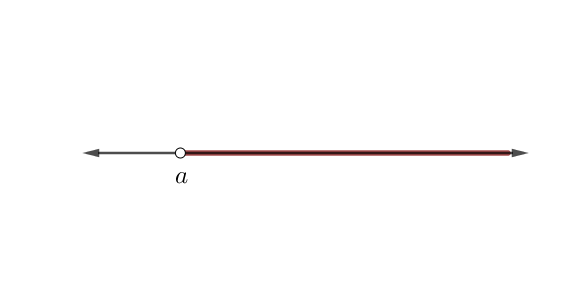
\includegraphics[scale=3.5]{imagens/semi-a-direita-aberta.png}

\end{figure}
\begin{center}
	Reta real
\end{center}

$$]-\infty,+\infty[ = \mathbb{R}$$
\begin{figure}[H]
	\centering
	
	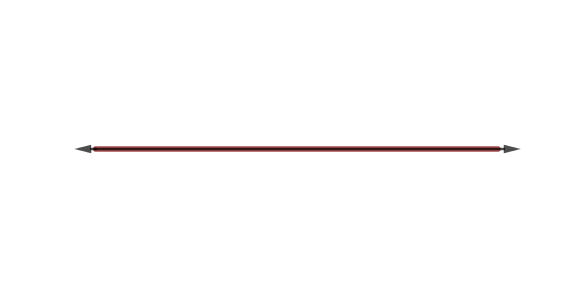
\includegraphics[scale=3.5]{imagens/reta-real.png}

\end{figure}

\end{itemize}


\chapter{Funções}

\section{Definição de Função}

Dados dois conjuntos $A$ e $B$, não vazios, uma relação $f$ de $A$ em $B$ recebe o nome de aplicação de $A$ em $B$ ou função de $A$ em $B$ se, e somente se, para todo $x \in A$ existe um só $y \in B $ tal que $(x,y) \in f$

\begin{figure}[H]
	\centering
	
	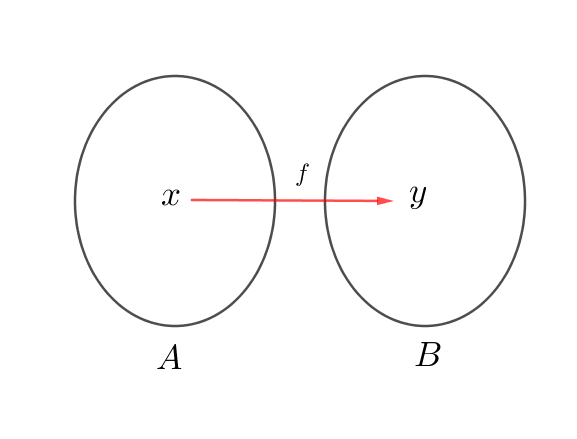
\includegraphics[scale=3.5]{imagens/funcao.png}

\end{figure}

\textbf{Exemplos:}

\begin{enumerate}

\item Dados os conjuntos $A = \{ -1\,;\,0\,;\,1\,;\,2\}$ e $B = \{0\,;\,1\,;\,2\,;\,3\}$, seja a relação $f$ de $A$ em $B$ expressa por $y=x+1$, com $x\in A$ e $y \in B$.

\begin{figure}[H]
	\centering
	
	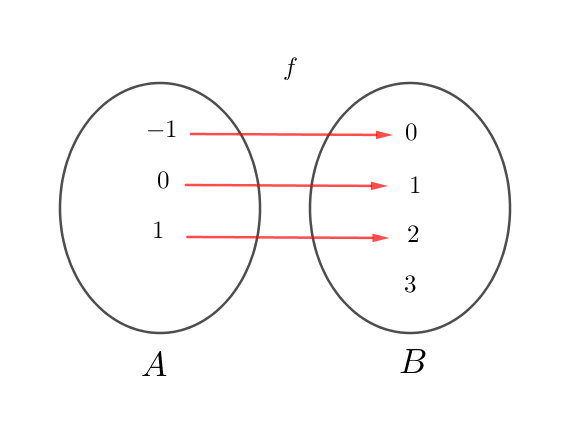
\includegraphics[scale=3.5]{imagens/funcao-ex1.png}

\end{figure}
\begin{itemize}
\item $x= -1 \, \Rightarrow \,y = -1+1 = 0  \, \Rightarrow (-1,0) \in f$
\item $x= 0 \, \Rightarrow \,y = 0+1 = 1 \, \Rightarrow (0,1) \in f $
\item $x= 1 \, \Rightarrow \,y = 1+1 = 2  \, \Rightarrow (1,2) \in f$

\item Todos os elementos de $A$ estão associados a elementos de $B$.
\item A cada elemento de $A$ está associado um único elemento de $B$.
\end{itemize}
Neste caso, a relação $f$ de $A$ em $B$ expressa por $y=x+1$ é uma função de $A$ em $B$.

\item Dados os conjuntos $A = \{ -1\,;\,1\,;\,3\}$ e $B = \{1\,;\,3\,;\,4\,;\,9\}$, seja a relação $f$ de $A$ em $B$ expressa por $y=x^2$, com $x\in A$ e $y \in B$.

\begin{figure}[H]
	\centering
	
	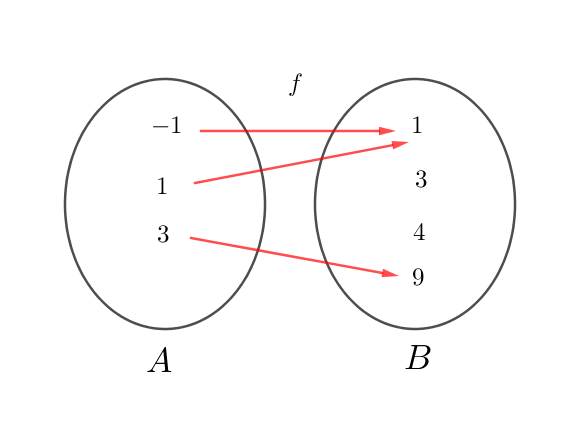
\includegraphics[scale=3.5]{imagens/funcao-ex2.png}

\end{figure}

\begin{itemize}
\item $x= -1 \, \Rightarrow \,y = (-1)^2 = 1 \, \Rightarrow (-1,1) \in f $
\item $x= 1 \, \Rightarrow \,y = (1)^2 = 1  \, \Rightarrow (1,1) \in f$
\item $x= 3 \, \Rightarrow \,y = (3)^2 = 9  \, \Rightarrow (3,9) \in f$

\item Todos os elementos de $A$ estão associados a elementos de $B$.
\item A cada elemento de $A$ está associado um único elemento de $B$.
\end{itemize}
Neste caso, a relação $f$ de $A$ em $B$ expressa por $y=x^2$ é uma função de $A$ em $B$.

\item Dados os conjuntos $A = \{ 0\,;\,1\,;\,2\}$ e $B = \{-1\,;\,0\,;\,1\,;\,4\}$, seja a relação $f$ de $A$ em $B$ expressa por $y^2=x$, com $x\in A$ e $y \in B$.

\begin{figure}[H]
	\centering
	
	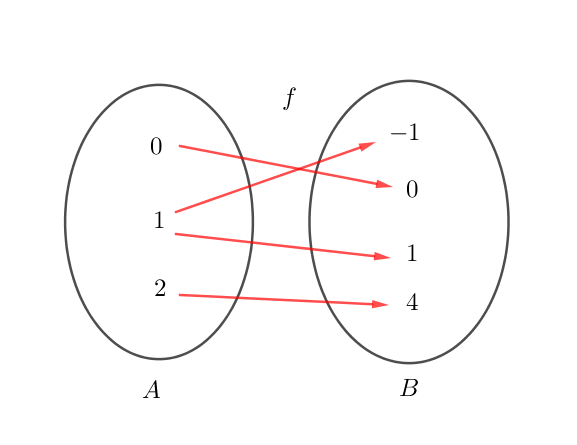
\includegraphics[scale=3.5]{imagens/funcao-ex3.png}

\end{figure}

\begin{itemize}
\item $x= 0 \, \Rightarrow \,y^2 = 0 = 0 \, \Rightarrow (0,0) \in f $
\item $x= 1 \, \Rightarrow \,y^2 = 1 = \pm 1  \, \Rightarrow (1,1)\, \text{e} \, (1,-1)\, \in f$
\item $x= 4 \, \Rightarrow \,y^2 = 4 = 2  \, \Rightarrow (4,2) \in f$

\item Todos os elementos de $A$ estão associados a elementos de $B$.
\item A cada elemento de $A$ \textbf{não} está associado \textbf{um único} elemento de $B$.
\end{itemize}
Neste caso, a relação $f$ de $A$ em $B$ expressa por $y^2=x$ \textbf{não} é uma função de $A$ em $B$.

\end{enumerate}

\section{Domínio, Contradomínio e Imagem de uma Função}

Toda função possui um domínio(digamos que são valores de partida) e uma imagem (valores de chegada).

\begin{figure}[H]
	\centering
	
	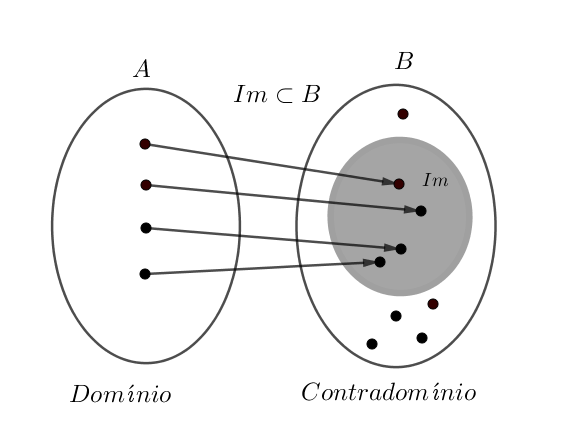
\includegraphics[scale=3.5]{imagens/domi-imag.png}

\end{figure}

\begin{itemize}

\item O domínio de uma função é o conjunto dos elementos de onde as setas partem.

\item A imagem de uma função é o conjunto dos elementos em que as setas chegam.

\item O contradomínio de uma função é o conjunto dos elementos possiveis em que as setas podem chegar.

\end{itemize}
\textbf{Observações:}
\begin{itemize}
\item O conjunto imagem está contido no contradomínio
\item As vezes é possivel que o conjunto imagem seja igual ao contradomínio $Im = B$.
\end{itemize}

\subsection{Pensando em função}

Podemos pensar em uma função como uma máquina. Com $x$ sendo os valores que entram (domínio)  e $y$ sendo os valores de saída (imagem) processados pela máquina. 

\begin{figure}[H]
	\centering
	
	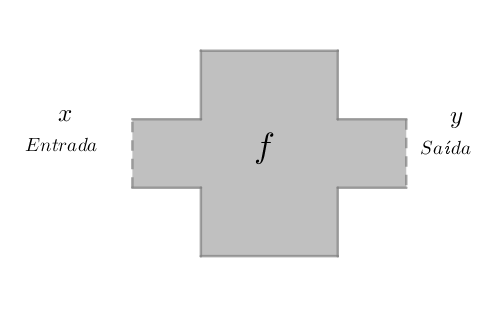
\includegraphics[scale=3.5]{imagens/pensa-funcao.png}

\end{figure}

\section{Gráfico de uma função}

O gráfico de uma função é o conjunto de pares ordenados $(x,y)$ 

\begin{figure}[H]
	\centering
	
	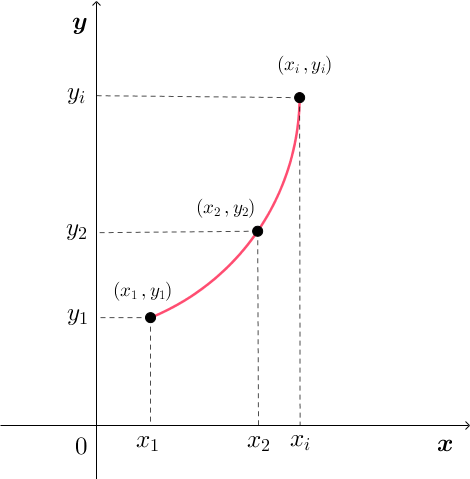
\includegraphics[scale=3.5]{imagens/graf-funcao.png}

\end{figure}
\chapter{Algebra}

%Potênciação

\section{Potênciação}
\subsection{Potência de Expoente Natural}

\newtheorem{definicao}{Definição}
\begin{definicao}
	Seja $a \in \mathbb{R} $ e $ n \in \mathbb{N}$. Potência de base $\textbf{a}$ e expoente $\textbf{n}$ é igual a:
\end{definicao}

\begin{equation*}
a^{n} = \overbrace{a \times a \times \cdots \times a  \times a}^n
\end{equation*}

\begin{equation*}
a^0 = 1 , a \neq 0
\end{equation*}


\textbf{Propriedades:}

Se $a$ e $b$ $ \in \mathbb{R}$ e  $n$ e $ m$ $ \in \mathbb{N}$, então valem as seguintes propriedades:
\begin{enumerate}
	\item $a^{m}a^{n} = a^{m+n}$
	\item $(a\cdot b)^n = a^n \cdot b^n$
	\item $\left(\dfrac{a}{b}\right)^n = \dfrac{a^n}{b^n} , b \neq 0$
	\item $(a^m)^n = a^{m\cdot n}$
\end{enumerate}
\textbf{Exemplos:}

\begin{itemize}

	\item $(-5)^0 = 1$
	\item $2^3 \cdot 2^2 = 2^{3+2} = 2^5 = 2\cdot 2\cdot 2\cdot 2\cdot 2 = 32$
	\item $(3\cdot 4)^2 = 3^2 \cdot 4^2 = 3\cdot 3 \cdot 4 \cdot 4 =9 \cdot 8 = 72$
	\item $\left(\dfrac{3}{2}\right)^2 = \dfrac{3^2}{2^3} = \dfrac{3\cdot 3}{2\cdot 2\cdot 2} =\dfrac{9}{8}$
	\item $(2^3)^2 = 2^{3 \cdot 2} = 2^6= 2\cdot 2\cdot 2\cdot 2\cdot 2 \cdot 2 = 64$
\end{itemize}


\subsection{Potência de Expoente Inteiro}

\newtheorem{definicao}{Definição}
\begin{definicao}
	Seja $a \in \mathbb{R}^* $ e $ n \in \mathbb{Z}$. Potência de base $\textbf{a}$ e expoente $\textbf{n}$ é igual a:	
\end{definicao}

$$ a^{-n} = \dfrac{1}{a^n}$$

\textbf{Propriedades:}

Se $a$ e $b$ $ \in \mathbb{R}^*$ e  $n$ e $ m$ $ \in \mathbb{Z}$, então valem as seguintes propriedades:

\begin{enumerate}

\item $\dfrac{a^m}{a^n} = a^{m-n}$
\item $a^{m}a^{n} = a^{m+n}$
\item $(a\cdot b)^n = a^n \cdot b^n$
\item $\left(\dfrac{a}{b}\right)^n = \dfrac{a^n}{b^n} $
\item $(a^m)^n = a^{m\cdot n}$

\end{enumerate}
\textbf{Exemplos:}

\begin{itemize}

	\item $(2)^{-2} = \dfrac{1}{2^2} = \dfrac{1}{4}$
	\item $ \dfrac{3^4}{3^2} = 3^{ 4-2} = 3^{2} = 9 $ 
	\item $ \dfrac{2^3}{2^5} = 2^{ 3-5} = 2^{-2} = \dfrac{1}{2^2} = \dfrac{1}{4}$
\end{itemize}

\subsection{Potência de Expoente Racional}

\newtheorem{definicao}{Definição}
\begin{definicao}
	Seja $a \in \mathbb{R}^*_+ $ e $ \dfrac{p}{q} \in \mathbb{Q} (p \in \mathbb{Z}$ e $ q \in \mathbb{N}^*_+)$. Potência de base $a$ e expoente $\dfrac{p}{q}$ é igual a:	
\end{definicao}

$$ a^{\frac{p}{q}} = \sqrt[q]{a^p} $$

\textbf{Propriedades:}

Se $a$ e $b$ $ \in \mathbb{R}^*_+$ e  $\dfrac{p}{q}$ e $\dfrac{r}{s} $ $ \in \mathbb{Z}$, então valem as seguintes propriedades:


\begin{enumerate}

\item $a^{\frac{p}{q}} \cdot a^{\frac{r}{s}} = a^{\frac{p}{q} + \frac{r}{s}}$

\item $\dfrac{a^{\frac{p}{q} }}{a^{\frac{r}{s} } } = a^{\frac{p}{q} - \frac{r}{s}}$

\item $(a\cdot b)^{\frac{p}{q}} = a^{\frac{p}{q}} \cdot b^{\frac{p}{q}}$

\item $\left(\dfrac{a}{b}\right)^{\frac{p}{q}} = \dfrac{a^{\frac{p}{q} }}{b^{\frac{p}{q} } }  $

\item $(a^{\frac{p}{q}})^{\frac{r}{s}} =  a^{\frac{p}{q} \cdot \frac{r}{s}   }$

\end{enumerate}


\textbf{Exemplos:}

\begin{itemize}

	\item $2^{\frac{1}{3}} \cdot 2^{\frac{2}{3}} = 2^{\frac{1}{3} + \frac{2}{3}} = 2^1 = 2$
	\item $\dfrac{3^{\frac{3}{5} }}{3^{\frac{1}{5} } } = 3^{\frac{3}{5} - \frac{1}{5}} = 3^{\frac{2}{5}}$
	\item $(5\cdot 4)^{\frac{1}{2}} = 5^{\frac{1}{2}} \cdot 4^{\frac{1}{2}} = \sqrt{5} \cdot \sqrt{4} = 2 \sqrt{5}$
	\item $\left(\dfrac{4}{3}\right)^{\frac{1}{2}} = \dfrac{4^{\frac{1}{2} }}{3^{\frac{1}{2} } } = \dfrac{\sqrt{4}}{\sqrt{3}} = \dfrac{2}{\sqrt{3}} = \dfrac{2}{\sqrt{3}} \cdot \dfrac{\sqrt{3}}{\sqrt{3}} = \dfrac{2\sqrt{3}}{3}  $
	\item $(6^{\frac{4}{3}})^{\frac{3}{2}} =  6^{\frac{4}{3} \cdot \frac{3}{2}   } = 6^{\frac{12}{6}}= 6^2 = 36$
\end{itemize}
\subsection{Potência de Expoente Irracional}

\newtheorem{definicao}{Definição}
\begin{definicao}
	Seja $a \in \mathbb{R} $ e $n$ um número irracional. Potência de base $a$ e expoente $n$ é  $a^n$.	
\end{definicao}

\textbf{Observações:}
\begin{itemize}
\item Se $a=0$ e $n$ é irracional e positivo, então:
$$ 0^n = 0$$ 
\item Se $a < 0 $ e $n$ é irracional e positivo, então $a^n$ não tem significado. Exemplos: $(-3)^{\sqrt{3}}$,$(-\sqrt{3})^{\sqrt{5}}$ e $(-9)^{\pi}$.
\item Se $n< 0$ então $0^n$ não tem significado.
\item Para as potências de expoente Irracional são válidas as propriedades anteriores.

\end{itemize}



\subsection{Potência de Expoente Real}
	
\newtheorem{definicao}{Definição}
\begin{definicao}
	Seja $a \in \mathbb{R}^*_+ $ e $ n \in \mathbb{R}$. Potência de base $a$ e expoente $n$ é  $a^n$.	
\end{definicao}

\textbf{Propriedades:}

Se $a$ e $b$ $ \in \mathbb{R}^*_+$ e  $n$ e $ m$ $ \in \mathbb{R}$, então valem as seguintes propriedades:

\begin{enumerate}
\item $ a^m \cdot a^n = a^{m+n}$
\item $\dfrac{a^m}{a^n} = a^{m-n}$
\item $(a\cdot b)^n = a^n \cdot b^n$
\item $\left(\dfrac{a}{b}\right)^n = \dfrac{a^n}{b^n} $
\item $(a^m)^n = a^{m\cdot n}$
\end{enumerate}
% Fim de Potênciação

\subsection{Radiciação}

Dados $a \in \mathbb{R}_+$ e $n \in \mathbb{N}, n \geq 1$, chama-se raiz n-ésima aritmética de $a$ o número real e não negativo $b$, tal que:
$$\sqrt[n]{a} = b \Leftrightarrow b^n = a$$


\textbf{Propriedades:}
Se $a$ e $b$ $ \in \mathbb{R}_+$ , $n$ e $ p$ $ \in \mathbb{N}$ e $m \in \mathbb{Z}$ então valem as seguintes propriedades:

\begin{enumerate}
\item $\sqrt[n]{a \cdot b} = \sqrt[n]{a} \cdot \sqrt[n]{b} $

\item $\sqrt[n]{\dfrac{a}{b}} = \dfrac{\sqrt[n]{a}}{\sqrt[n]{b}} ,\,\,\, b > 0$

\item $(\sqrt[n]{a})^m = \sqrt[n]{a^m}$

\item $\sqrt[n]{a^m} = \sqrt[n\cdot p]{a^{m\cdot p}}$

\item $\sqrt[p]{\sqrt[n]{a^m}} = \sqrt[p \cdot n]{a^m}$
\end{enumerate}

%Produtos Notaveis
\newpage
\section{Produtos Notáveis}

\subsection{Quadrado da Soma Entre Dois Termos}

	
	$$(a+b)^{2} = (a+b)(a+b) = a\cdot a + a\cdot b + b\cdot a + b\cdot b $$
	
	
	$$a^2+2ab+b^2$$
	
\begin{figure}[H]
	\centering
	
	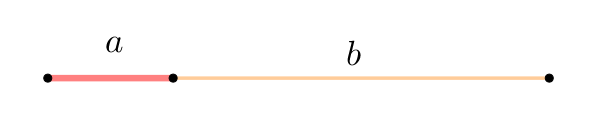
\includegraphics[scale=3.5]{imagens/soma-quadrado1.png}

\end{figure}

\begin{figure}[H]
	\centering
	
	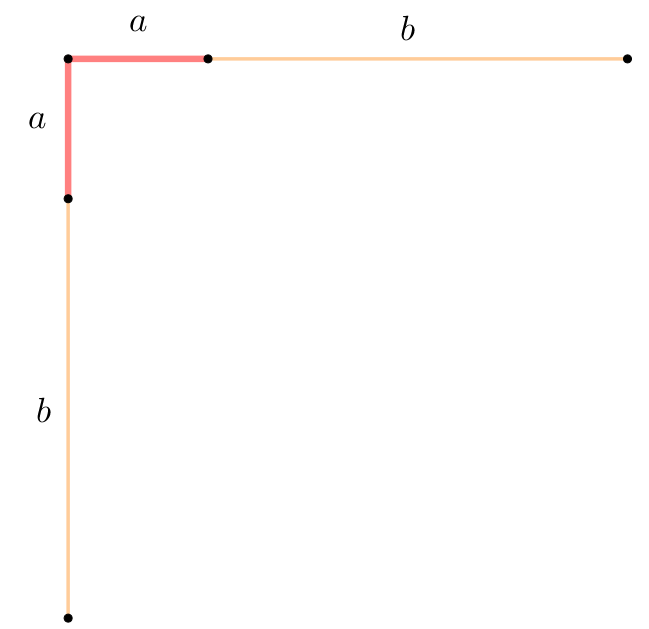
\includegraphics[scale=3.5]{imagens/soma-quadrado2.png}

\end{figure}
	
\begin{figure}[H]
	\centering
	
	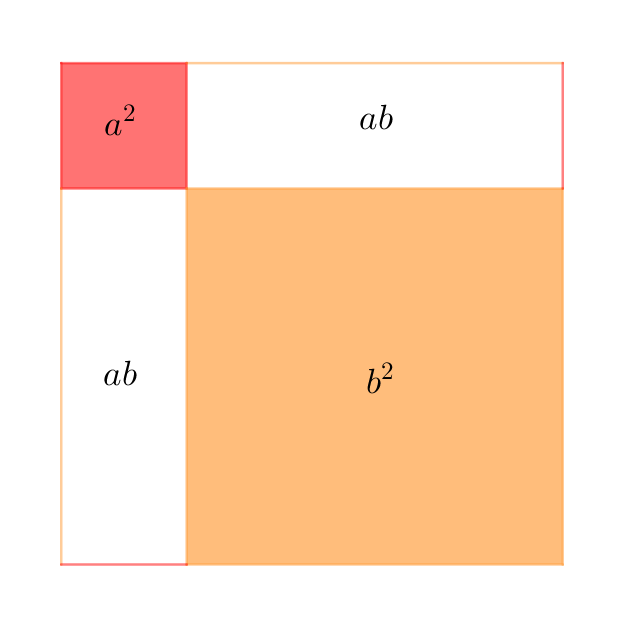
\includegraphics[scale=3.5]{imagens/soma-quadrado.png}

\end{figure}
	
\subsection{Quadrado da Diferença Entre dois Termos}

	$$(a-b)^{2} = (a-b)(a-b) = a\cdot a - a\cdot b - b\cdot a + b\cdot b $$
	
	$$a^2-2ab+b^2$$
	
\subsection{Diferença de Quadrados}

	$$(a+b)(a-b) = a\cdot a - a\cdot b + b\cdot a + b\cdot b $$
	
	$$a^{2}-b^{2}$$
	
\subsection{Cubo da Soma Entre Dois Termos}

	$$(a+b)^{3} = (a+b)(a+b)^{2} = (a+b)(a^{2}+2ab+b^{2}) = a\cdot a^{2} + 2a\cdot a \cdot b + a\cdot b^{2} + b\cdot a^{2} + 2\cdot a \cdot b\cdot b + b\cdot b^{2} $$
	
	$$a^{3} + 3a^{2}b + 3ab^{2}+b^{3}$$

\subsection{Cubo da Diferença Entre Dois Termos}

$$(a-b)^{3} = (a-b)(a-b)^{2} = (a-b)(a^{2}-2ab+b^{2}) = a a^{2} - a2ab + a\cdot b^{2} - b\cdot a^{2} + 2\cdot a \cdot b\cdot b - b\cdot b^{2} $$
	
	$$a^{3} - 3a^{2}b + 3ab^{2} - b^{3}$$
	
\section{Técnicas de Fatoração}


\subsection{Termo em Evidência}

	$$2x^{2}+2xy = 2x(x+y)$$
	
\subsection{Agrupamento}

	$$ax+ 5a + 5x + 25$$
	$$a(x+5)+5(x+5)$$
	$$(x+5)(a+5)$$
	
\subsection{Quadrado perfeito}

	$$x^{2} + 8x +16 = x^{2}+2\cdot 4\cdot x + 4^{2} = (x+4)^{2}$$
	
	
\subsection{Diferença de Quadrados}

	$$x^{2} - 25 = x^{2} - 5^{2} = (x+5)(x-5)$$
	
\subsection{Soma de Dois Cubos}

	$$x^{3}+y^{3} = (x+y)(x^{2} - xy + y^{2})$$
	
\subsection{Diferença de Dois Cubos}

	$$x^{3} - y^{3} = (x-y)(x^{2} + xy + y^{2})$$
	
\subsection{Fatorações Sucessivas}

	$$3x^{2} - 75 = 3x^{2} - 3\cdot 25 = 3(x^{2} - 25) = 3(x^{2} - 5^{2}) = 3(x+5)(x-5)$$
	
\chapter{Geometria Analitica}

\section{Noções Iniciais}
\subsection{Distância Entre Dois Pontos}

Dados dois pontos $A(x_a\, , y_a)$ e $B(x_b\, , y_b)$ a distância entre $A$ e $B$ é dada por:
$$d_{AB} = \sqrt{(x_a - x_b)^2 + (y_a - y_b)^2}$$


\begin{figure}[H]
	\centering
	
	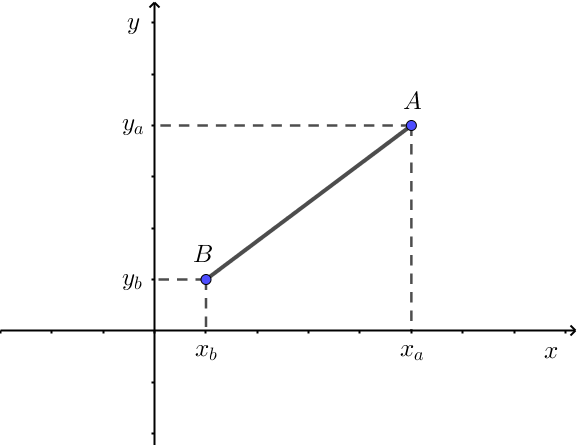
\includegraphics[scale=3.5]{imagens/distanciaab.png}

\end{figure}

\newtheorem{proof}{Demonstração}
\begin{proof}
Vamos demonstrar a formula da distância entre dois pontos.
Considere o triângulo $ABC$ na imagem abaixo:
\end{proof}

\begin{figure}[H]
	\centering
	
	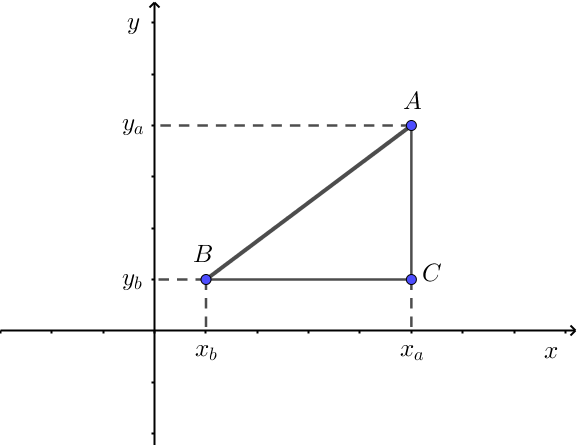
\includegraphics[scale=3.5]{imagens/distanciad.png}

\end{figure}
\begin{center}
Aplicando o teorema de Pitágoras no triângulo $ABC$ temos:
\end{center}


$$d_{AB}^2 = d_{BC}^2 + d_{AC}^2$$
\begin{center}
Do triângulo $ABC$ temos  que $d_{BC} = (x_a - x_b)$ e $d_{AC} = (y_a - y_b)$ então:
\end{center}

$$d_{AB}^2 ={(x_a - x_b)}^2 + {(y_a - y_b)}^2   $$

$$d_{AB} = \sqrt{{(x_a - x_b)}^2 + {(y_a - y_b)}^2}$$


\subsection{Circunferência}

Uma circunferência é o conjunto de pontos no plano que estão a uma certa distância $r$ de um ponto dado $( a, b )$.
Um ponto $( x, y )$ pertence a circunferência
de centro $( a, b )$ e raio $r$ se e somente se satisfaz a equação:

$${(x - a)}^2 + {(y - b)}^2=r^2$$
\begin{figure}[H]
	\centering
	
	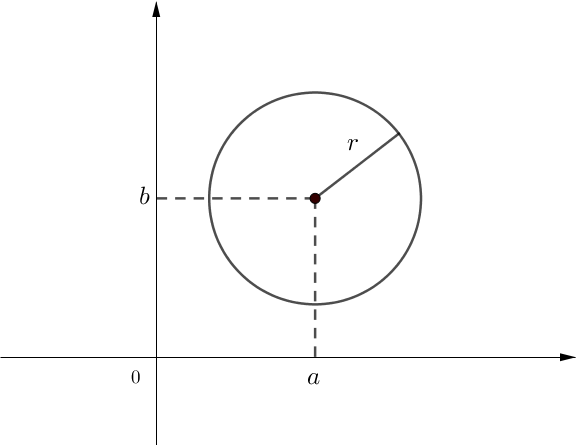
\includegraphics[scale=3.5]{imagens/circunferencia1.png}

\end{figure}
\newtheorem{proof}{Demonstração}
\begin{proof}
Vamos demonstrar a equação da circunferência.
Considere a seguinte imagem abaixo:
\end{proof}

\begin{figure}[H]
	\centering
	
	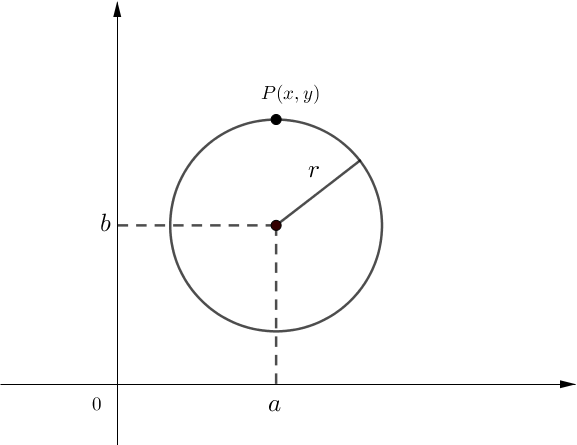
\includegraphics[scale=3.5]{imagens/circunferencia2.png}

\end{figure}
\begin{center}
Usando a definição de circunferência, temos que um ponto $P(x,y)$ pertence a circunferência se e somente se a distância dele até o centro $C(a,b)$ é igual a $r$. Escrevendo essa relação, temos:
\end{center}

$$ d_{PC} = r $$

\begin{center}

Usando a equação da distância entre dois pontos e substituindo na equação acima, temos:

\end{center}
$$\sqrt{{(x - a)}^2 + {(y - b)}^2} = r $$

\begin{center}

elevando ao quadrado os dois lados da equação acima, temos:

\end{center}

$$ {(x - a)}^2 + {(y - b)}^2 = r^2$$
\chapter{Trigonometria}

\section{Razões Trigonométricas no Triângulo Retângulo}

\subsection{Triângulo Retângulo}


Um Triângulo é dito retângulo quando um de seus ângulos internos é reto. 


\begin{figure}[H]
	\centering
	
	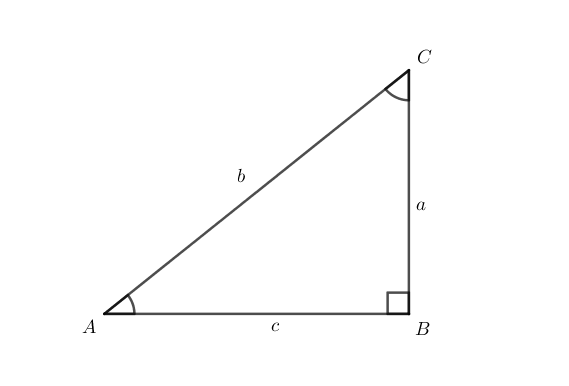
\includegraphics[scale=3.5]{imagens/triangulo-retangulo.png}

\end{figure}

\subsection{Teorema de Pitágoras}
\newtheorem{teorema}{Teorema}
\begin{teorema}
	O quadrado da Hipotenusa é igual à soma do quadrado dos catetos.
\end{teorema}

		$$a^{2}=b^{2}+c^{2}$$ 
		
\newtheorem{proof}{Demonstração}
\begin{proof}
    Vamos demonstrar o teorema de Pitágoras.
\end{proof}

Considere o quadrado de lado $ a $ inscrito no quadrado de lado $ b+c $.

\begin{figure}[H]
	\centering
	
	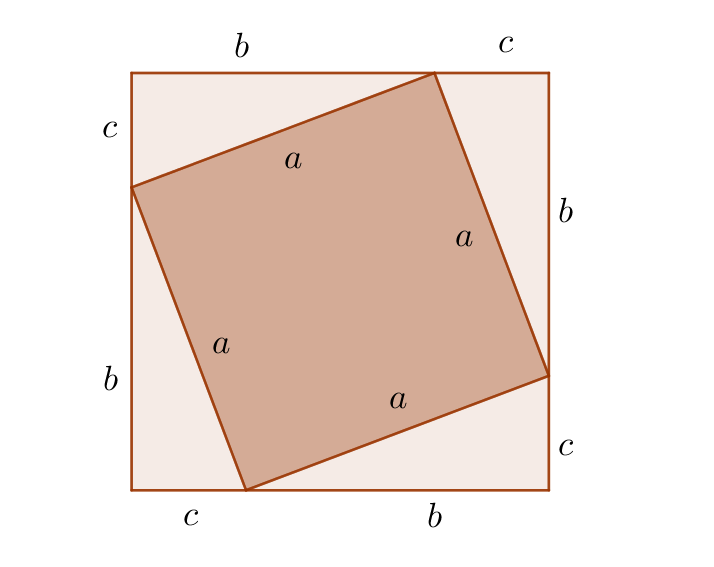
\includegraphics[scale=3.5]{imagens/pitagoras.png}

\end{figure}

A partir da figura acima percebe-se que a área do quadrado $a$ é igual a área do quadrado $b+c$ menos a área dos 4 triângulos de lados $b$ e $c$. Escrevendo essa relação, temos:
$$a^{2} = (b+c)^2 - 4\left(\dfrac{bc}{2}\right)$$

$$a^{2} = b^{2} + 2bc + c^{2} - 2bc$$

$$ a^{2} = b^{2}+c^{2}  $$

\textbf{Observação:}
$\left(\frac{bc}{2}\right)$ é a área do triângulo retângulo de catetos $b$ e $c$.

\subsection{Seno, Cosseno e Tangente}

Considere o triângulo retângulo abaixo:

\begin{figure}[H]
	\centering
	
	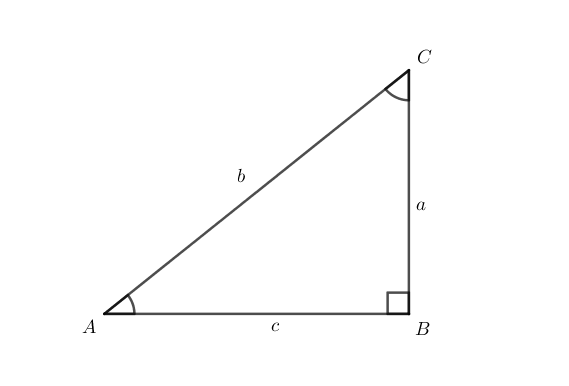
\includegraphics[scale=3.5]{imagens/triangulo-retangulo.png}

\end{figure}

\subsubsection{Seno}
O seno de um ângulo agudo é a razão entre o cateto oposto a esse ângulo e a hipotenusa
$$\sen\hat{A} = \dfrac{a}{b}$$

\subsubsection{Cosseno}
O cosseno de um ângulo agudo é a razão entre o cateto adjacente a esse ângulo e a hipotenusa
$$\cos \hat{A} = \dfrac{c}{b}$$

\subsubsection{Tangente}
A tangente de um ângulo agudo é a razão entre o cateto oposto a esse ângulo e o cateto adjacente.
$$\tg \hat{A} = \dfrac{a}{c}$$

\subsection{Relação Fundamental da Trigonometria}

considere o seguinte triângulo retângulo:

\begin{figure}[H]
	\centering
	
	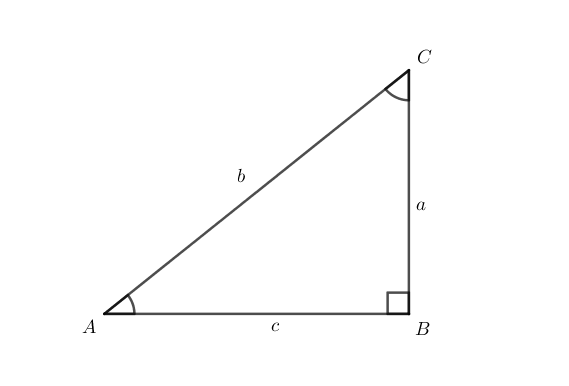
\includegraphics[scale=3.5]{imagens/triangulo-retangulo.png}

\end{figure}

\newtheorem{proof}{Demonstração}
\begin{proof}
Vamos demonstrar a relação fundamental da Trigonometria.
\end{proof}

$$\sen\hat{A} = \dfrac{a}{b} \, \Rightarrow a = b \sen\hat{A} $$


$$\cos \hat{A} = \dfrac{c}{b} \, \Rightarrow c = b \cos \hat{A}$$

Pelo teorema de Pitágoras, temos $ b^{2}=a^{2}+c^{2}$. Substituindo os valores:
$$ b^{2}=( b \sen\hat{A} )^{2}+(b \cos \hat{A})^{2}$$
$$b^{2}= b^{2} \sen^{2}\hat{A} +b^{2} \cos^{2} \hat{A}$$
Dividindo de ambos os lados da equação por $ b^{2}$ temos:

$$\sen^{2}\hat{A} + \cos^{2} \hat{A} = 1 $$

\subsection{Ângulos Complementares}


considere o Triângulo retângulo abaixo:

\begin{figure}[H]
	\centering
	
	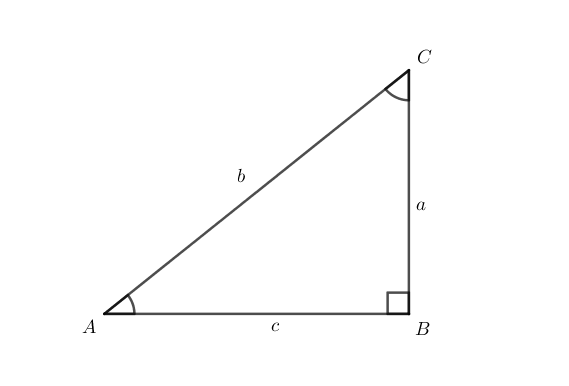
\includegraphics[scale=3.5]{imagens/triangulo-retangulo.png}

\end{figure}


$$
\begin{cases}
\hat{A}+\hat{B}+\hat{C}=180̣^{\circ}
\hat{B} = 90^{\circ}\\
\hat{A} + \hat{C} = 90^{\circ}
\end{cases}
$$

Dizemos que $\hat{A} $ e $ \hat{C} $ são complementares, pois a soma dos dois é igual à $90^{\circ}$. Com isso decorre as seguintes relações:

$$\sen\hat{A} = \dfrac{a}{b}$$

$$\cos\hat{C} = \dfrac{a}{b}$$
\centering
\xymatrix{
*+[F-:<3pt>]{
\sen\hat{A} = \cos\hat{C}}
\\
\\}



$$\cos\hat{A} = \dfrac{c}{b}$$
$$\sen\hat{C} = \dfrac{c}{b}$$
\centering
\xymatrix{
*+[F-:<3pt>]{
\cos\hat{A} = \sen\hat{C} }
\\}

\newpage









%\begin{figure}[H]
%	\centering
%	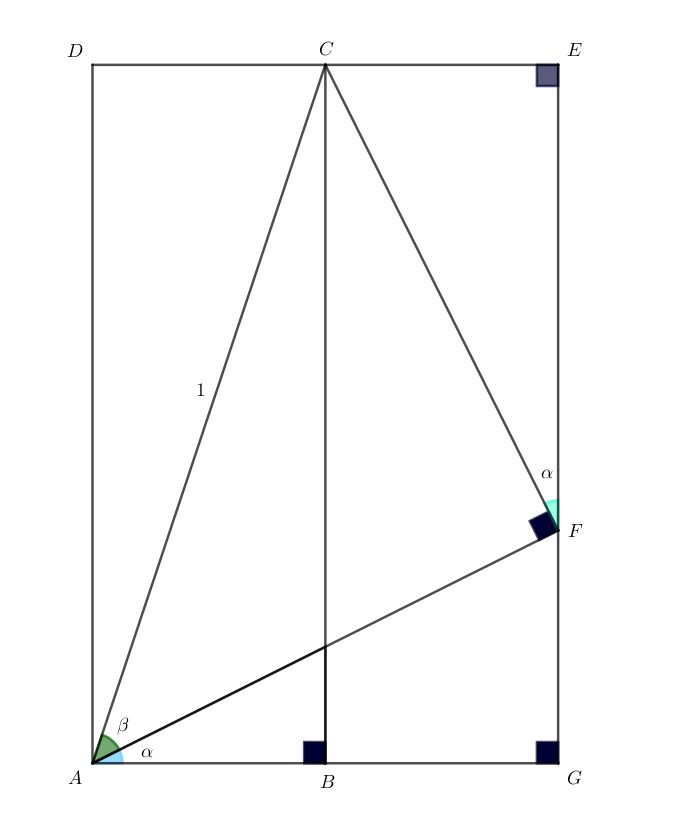
\includegraphics[scale=3.5]{imagens/soma-seno-cosseno.png}
%\end{figure}



\end{document}
